%
% ---------- header -----------------------------------------------------------
%
% project       kaneton
%
% license       kaneton
%
% file          /home/mycure/kane...cture/kernels/future/devices/devices.tex
%
% created       julien quintard   [wed may 16 19:28:59 2007]
% updated       julien quintard   [mon apr 13 03:30:06 2009]
%

%
% ---------- setup ------------------------------------------------------------
%


%
% path
%

\def\path{../../../..}

%
% template
%

%
% ---------- header -----------------------------------------------------------
%
% project       kaneton
%
% license       kaneton
%
% file          /home/mycure/kaneton/view/template/lecture.tex
%
% created       julien quintard   [wed may 16 18:17:26 2007]
% updated       julien quintard   [sun may 18 23:23:40 2008]
%

%
% class
%

\documentclass[8pt]{beamer}

%
% packages
%

\usepackage{pgf,pgfarrows,pgfnodes,pgfautomata,pgfheaps,pgfshade}
\usepackage[T1]{fontenc}
\usepackage{colortbl}
\usepackage{times}
\usepackage{amsmath,amssymb}
\usepackage{graphics}
\usepackage{graphicx}
\usepackage{color}
\usepackage{xcolor}
\usepackage[english]{babel}
\usepackage{enumerate}
\usepackage[latin1]{inputenc}
\usepackage{verbatim}
\usepackage{aeguill}

%
% style
%

\usepackage{beamerthemesplit}
\setbeamercovered{dynamic}

%
% verbatim stuff
%

\definecolor{verbatimcolor}{rgb}{0.00,0.40,0.00}

\makeatletter

\renewcommand{\verbatim@font}
  {\ttfamily\footnotesize\selectfont}

\def\verbatim@processline{
  {\color{verbatimcolor}\the\verbatim@line}\par
}

\makeatother

%
% -
%

\renewcommand{\-}{\vspace{0.4cm}}

%
% date
%

\date{\today}

%
% logos
%

\pgfdeclareimage[interpolate=true,width=34pt,height=18pt]
                {epita}{\path/logo/epita}
\pgfdeclareimage[interpolate=true,width=49pt,height=18pt]
                {upmc}{\path/logo/upmc}
\pgfdeclareimage[interpolate=true,width=25pt,height=18pt]
                {lse}{\path/logo/lse}

\newcommand{\logos}
  {
    \pgfuseimage{epita}
  }

%
% institute
%

\institute
{
  \inst{1} kaneton microkernel project
}

%
% table of contents at the beginning of each section
%

\AtBeginSection[]
{
  \begin{frame}<beamer>
   \frametitle{Outline}
    \tableofcontents[current]
  \end{frame}
}

%
% table of contents at the beginning of each subsection
%

\AtBeginSubsection[]
{
  \begin{frame}<beamer>
   \frametitle{Outline}
    \tableofcontents[current,currentsubsection]
  \end{frame}
}


%
% title
%

\title{Devices}

%
% document
%

\begin{document}

%
% title frame
%

\begin{frame}
  \titlepage
\end{frame}

%
% outline frame
%

\begin{frame}
  \frametitle{Outline}

  \tableofcontents
\end{frame}

  % -)

\section{Hardware memory access}
\begin{frame}
  \frametitle{Minimal components and buses}
  \begin{center}
    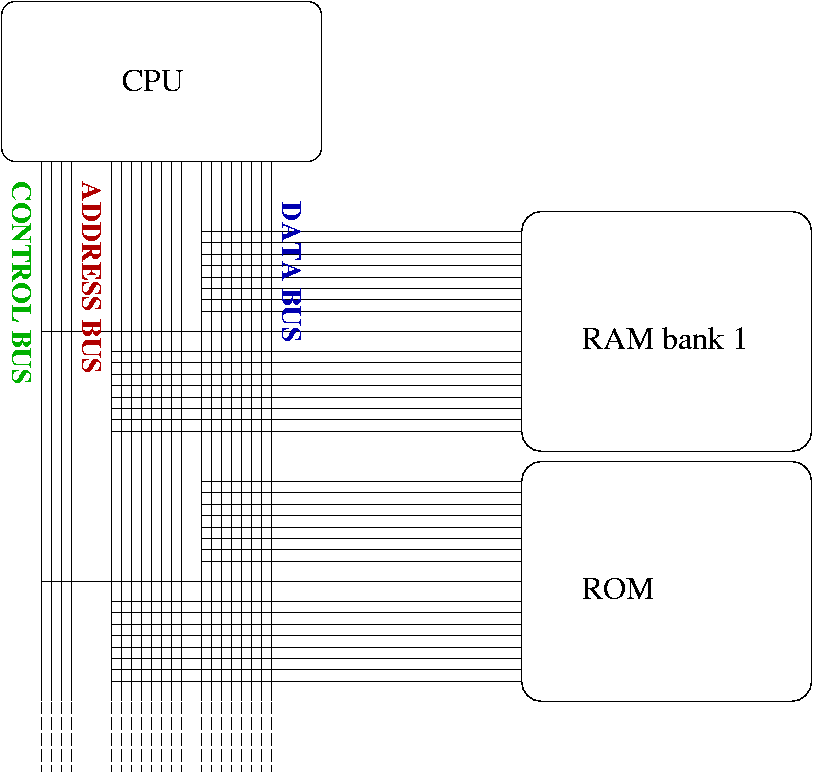
\includegraphics[width=150pt,height=150pt]{figures/arch-basic}
  \end{center}
\end{frame}


\subsection{Memory accesses}
\begin{frame}
  \frametitle{Memory accesses}
  \begin{center}
    \begin{overlayarea}{10cm}{10cm}
      \only<1>{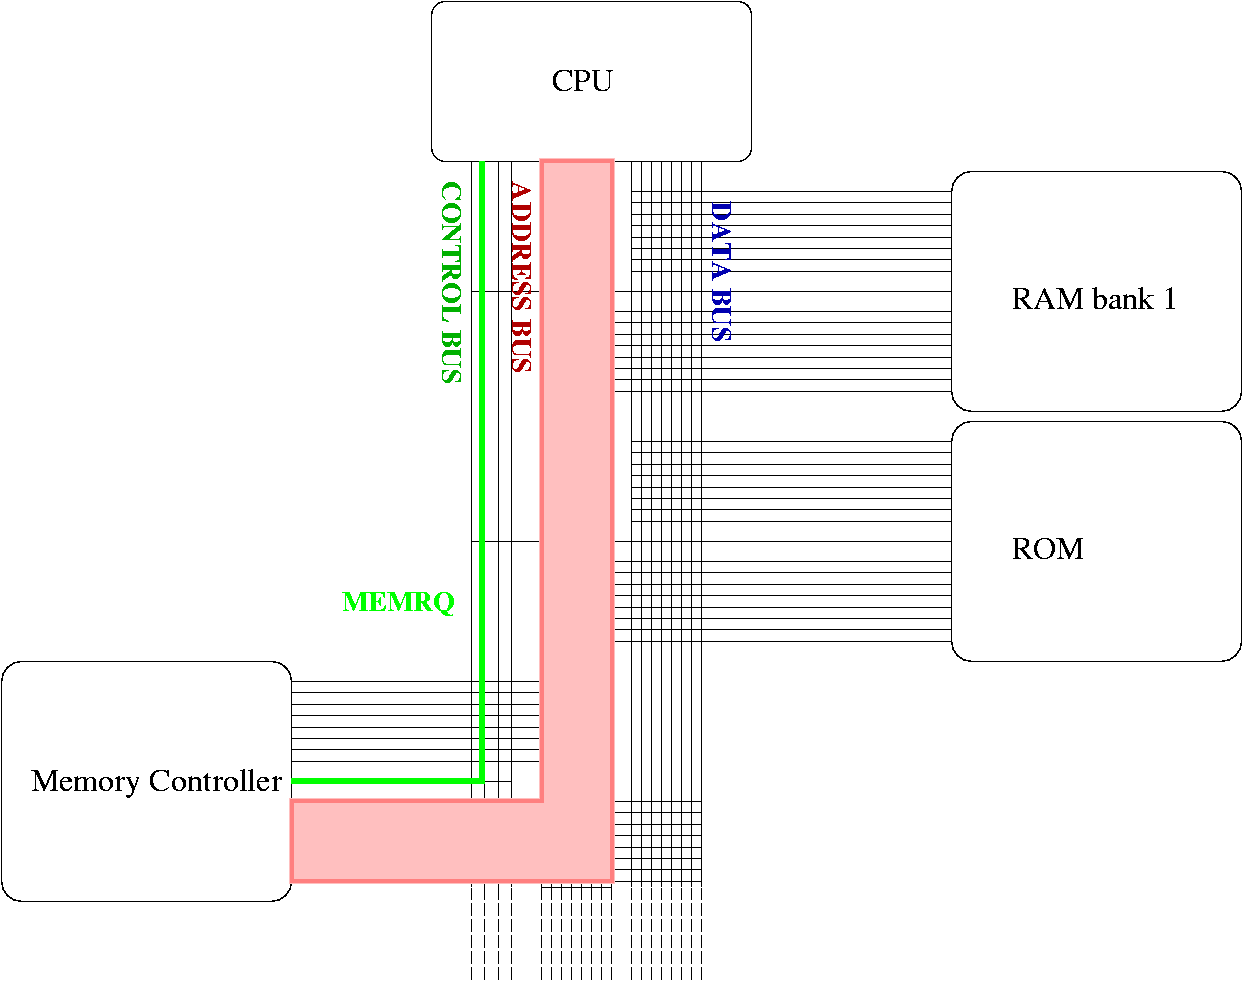
\includegraphics[width=240pt,height=200pt]{figures/memory-access-step1}}
      \only<2>{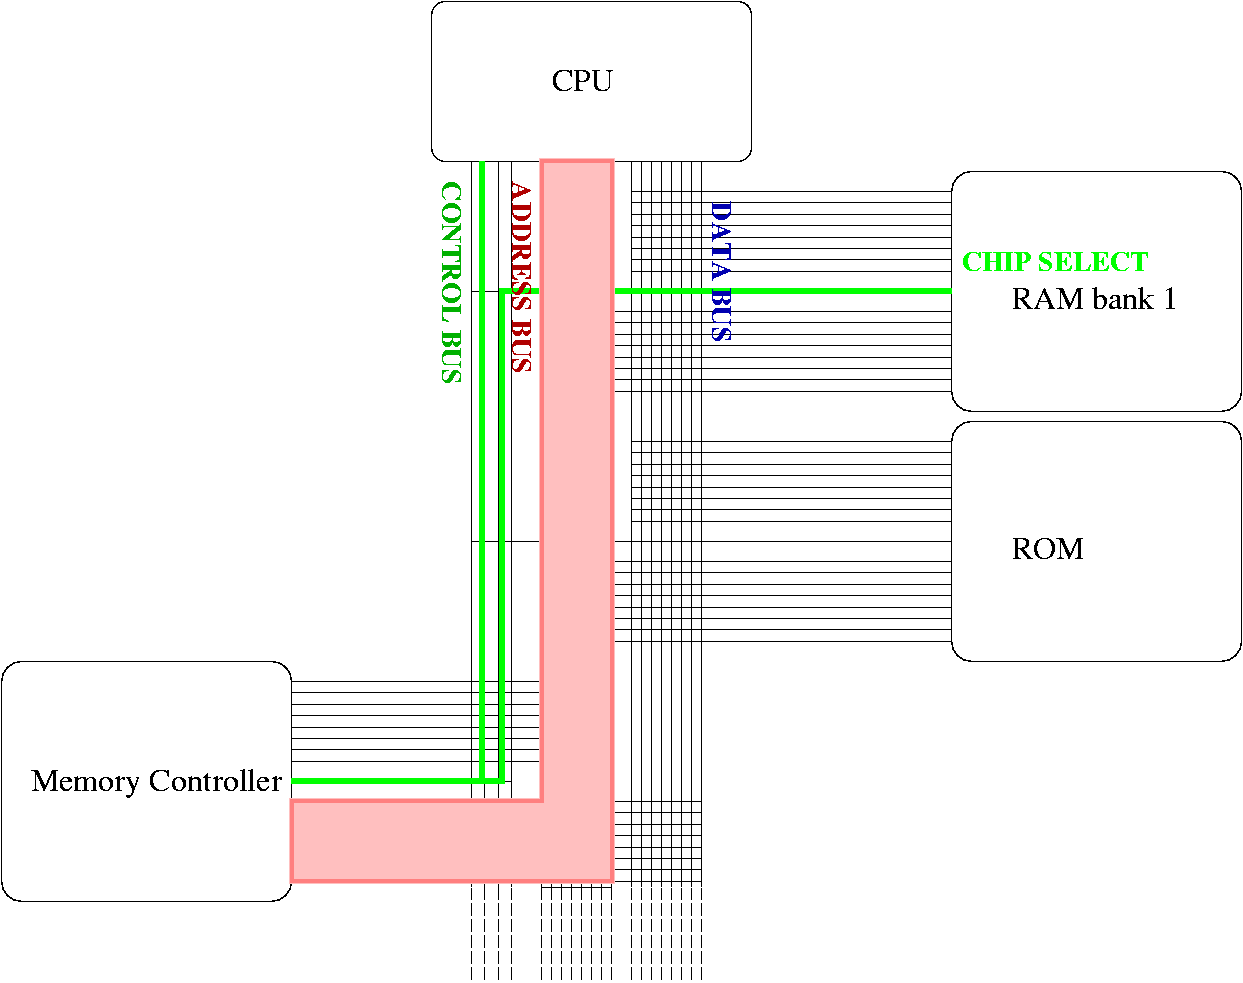
\includegraphics[width=240pt,height=200pt]{figures/memory-access-step2}}
      \only<3>{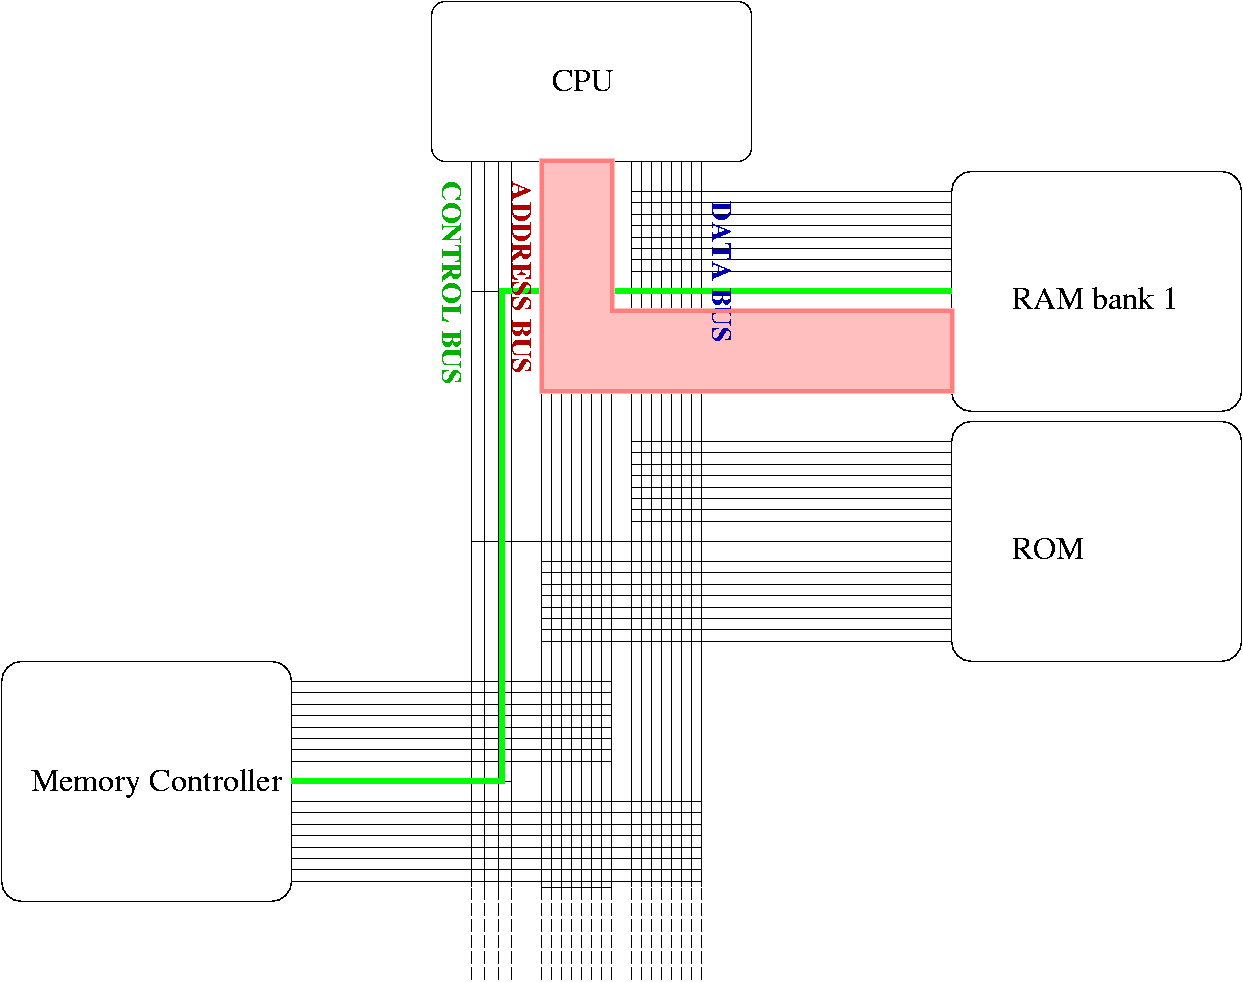
\includegraphics[width=240pt,height=200pt]{figures/memory-access-step3}}
      \only<4>{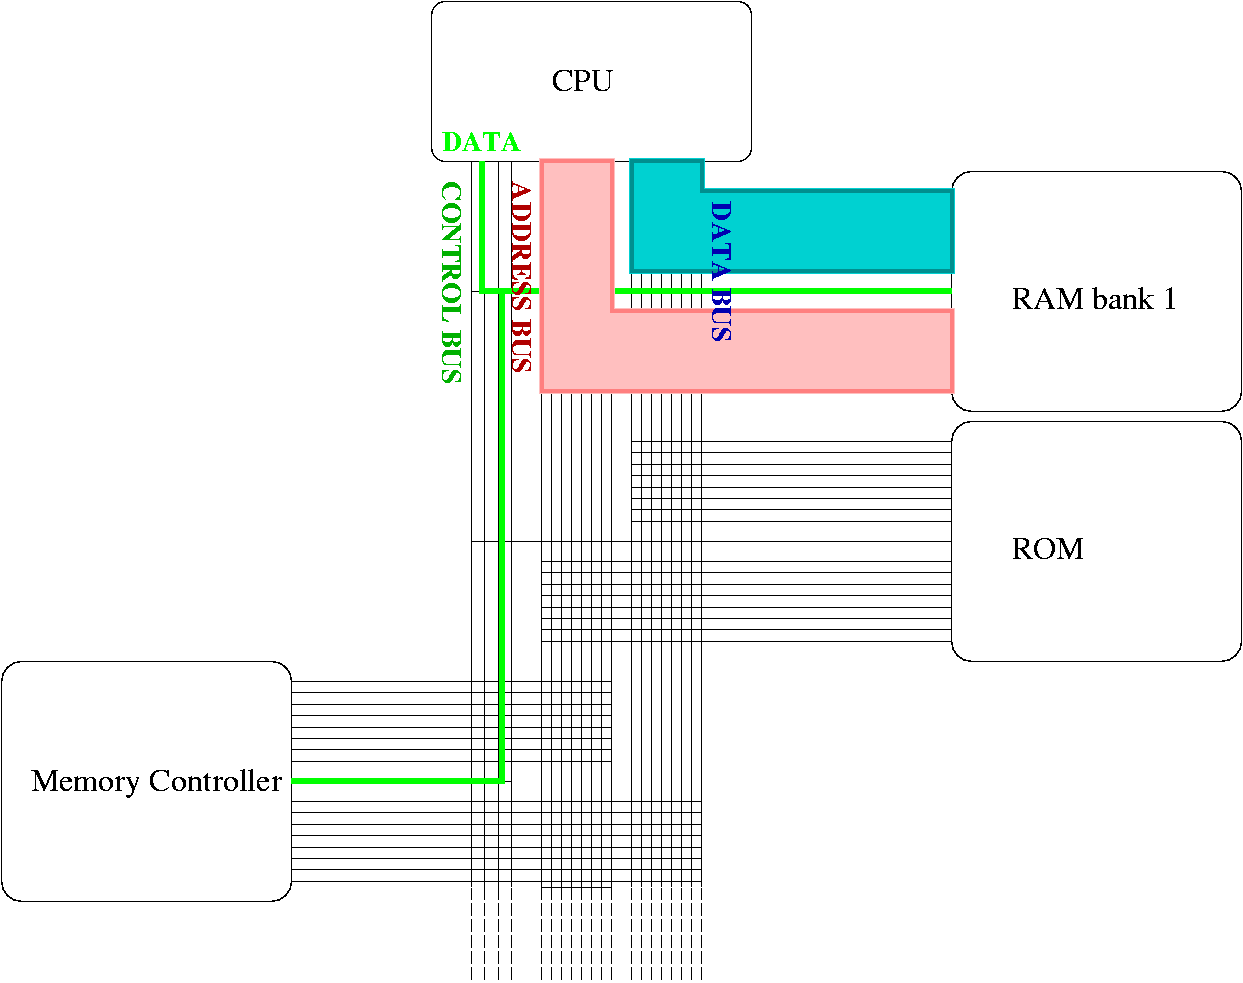
\includegraphics[width=240pt,height=200pt]{figures/memory-access-step4}}
    \end{overlayarea}
  \end{center}
\end{frame}

% -)

\subsection{Memory controller}
\begin{frame}
  \frametitle{Memory controller}
  \begin{center}
    \only<1>{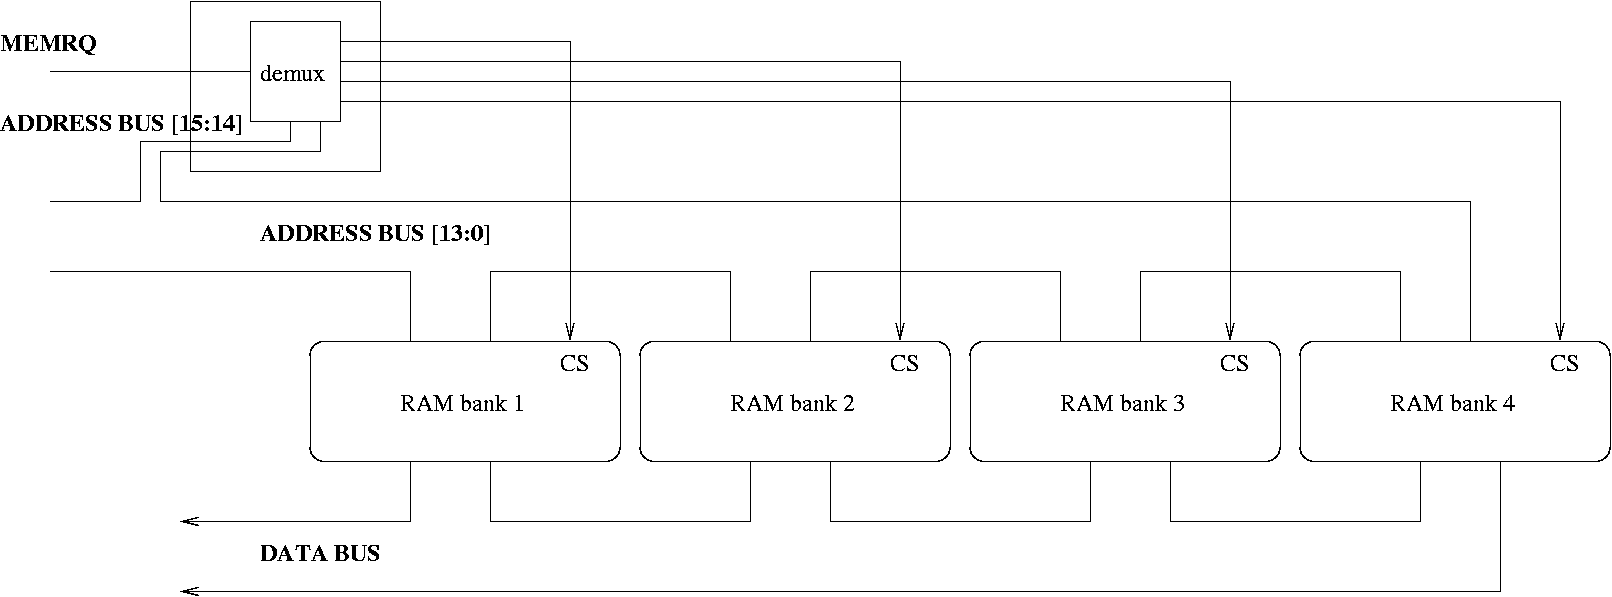
\includegraphics[width=300pt,height=110pt]{figures/memory-controller}}
  \end{center}
\end{frame}

% -)

\subsection{Misaligned Memory access}
\begin{frame}
\frametitle{Misaligned memory access}
  \begin{itemize}
    \item Memory access are not every time aligned.
    \item For instance "movl (\$0xABCD57), \%eax".
    \item Some architecture doesn't support unaligned memory access, the
    processor raise an exception (Sparc).
    \item Hopufully (or not) x86 supports unaligned memory access.
  \end{itemize}
\end{frame}

\begin{frame}
  \frametitle{Misaligned memory access}
  \begin{center}
\begin{overlayarea}{10cm}{10cm}
    \only<1>{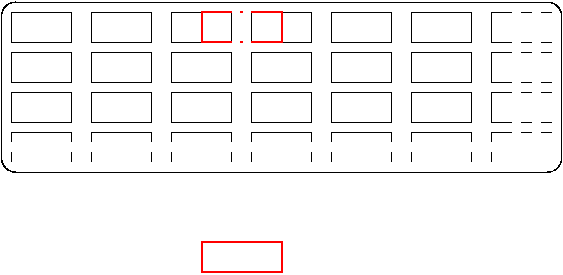
\includegraphics[width=300pt,height=150pt]{figures/unaligned-step1}}
    \only<2>{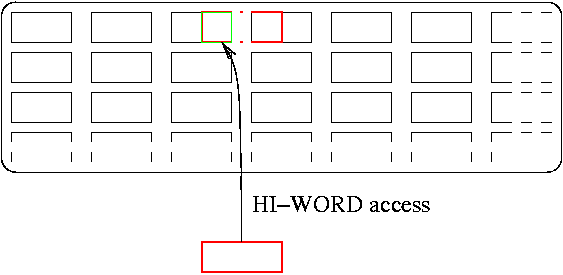
\includegraphics[width=300pt,height=150pt]{figures/unaligned-step2}}
    \only<3>{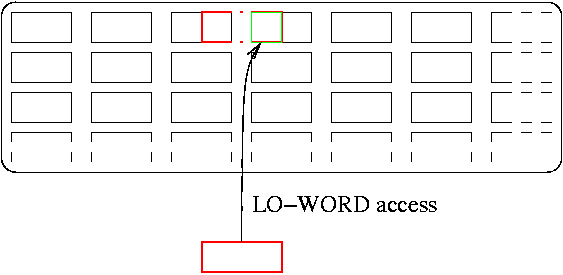
\includegraphics[width=300pt,height=150pt]{figures/unaligned-step3}}
    \only<4>{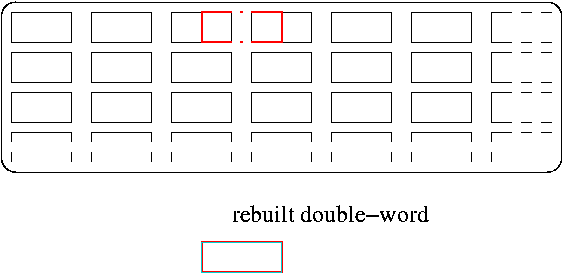
\includegraphics[width=300pt,height=150pt]{figures/unaligned-step4}}
\end{overlayarea}
  \end{center}
\end{frame}

\section{Devices}

\subsection{What is a device?}
\begin{frame}
\begin{itemize}
  \item A device is a piece of hardware connected on a computer via a
        bus.
  \item It can be a wired bus or over the air, like bluetooth.
  \item A device can make actions and has different status.
  \item To store all those informations device use registers.
  \item Devices need interrupts in order to notify the computer. It's
  for synchronous actions.
\end{itemize}
\end{frame}
\subsection{Register}
\begin{frame}
\frametitle{Devies Registers}
\begin{itemize}
        \item Registers can be access using an address on the device.
        \item Sometimes the device memory is mapped on the computer
        physical memory, sometime it required to use some I/O
        instrucitons.
        \item There is 2 types of registers:
        \begin{itemize}
          \item Actions registers, ofen write only (but ca be RW),
          writing to those registers do an action.
          \item Status registers, read only. This is ofen the result of
          an action.
        \end{itemize}
\end{itemize}
\end{frame}


\section{Different way to get in...}
\subsection{PIO}

\begin{frame}
        \frametitle{PIO}
        \begin{itemize}
        \item Programmed Input Output.
        \item Use instruction in{b,w,l} and out{b,w,l}.
        \item Very slow.
        \item Takes a lot of CPU loads.
        \item The processor cannot do something else when data are
        transfering.
        \end{itemize}
\end{frame}

\begin{frame}
\begin{center}
\begin{overlayarea}{10cm}{10cm}
\only<1>{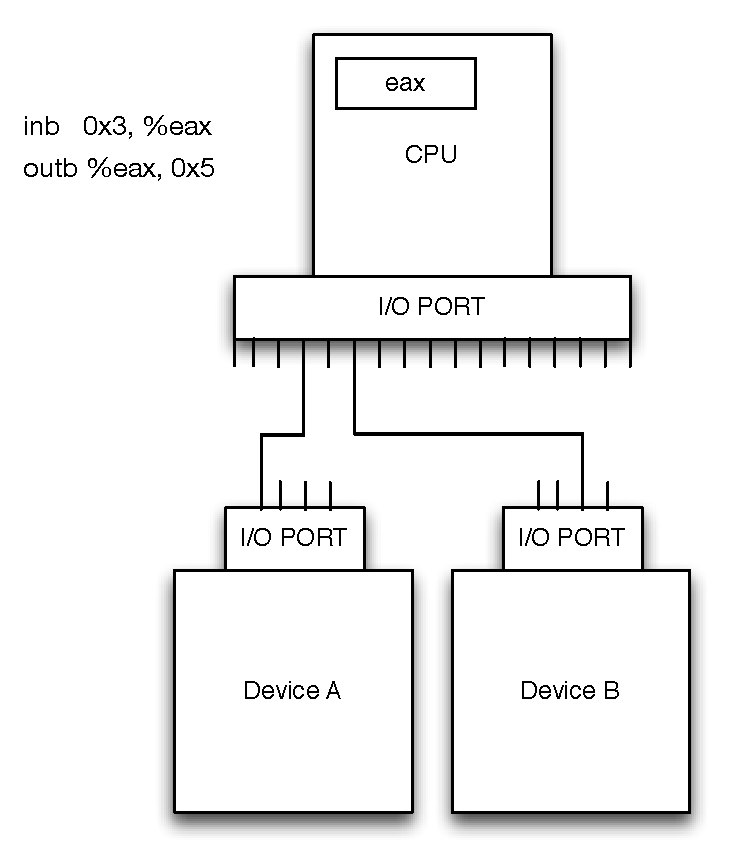
\includegraphics[height=225pt]{figures/ioport_1.pdf}}
\only<2>{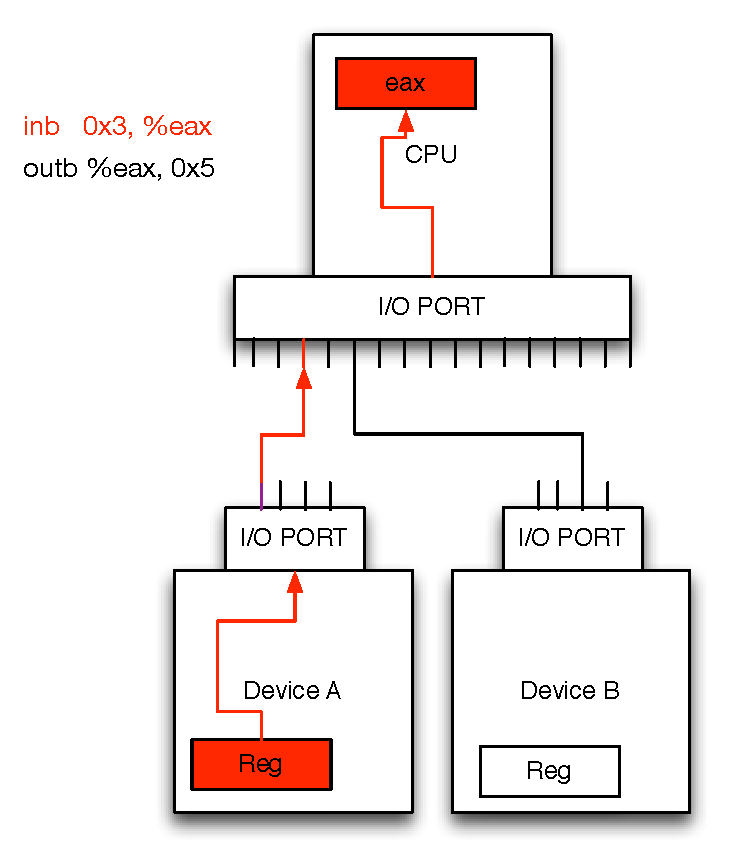
\includegraphics[height=225pt]{figures/ioport_2.pdf}}
\only<3>{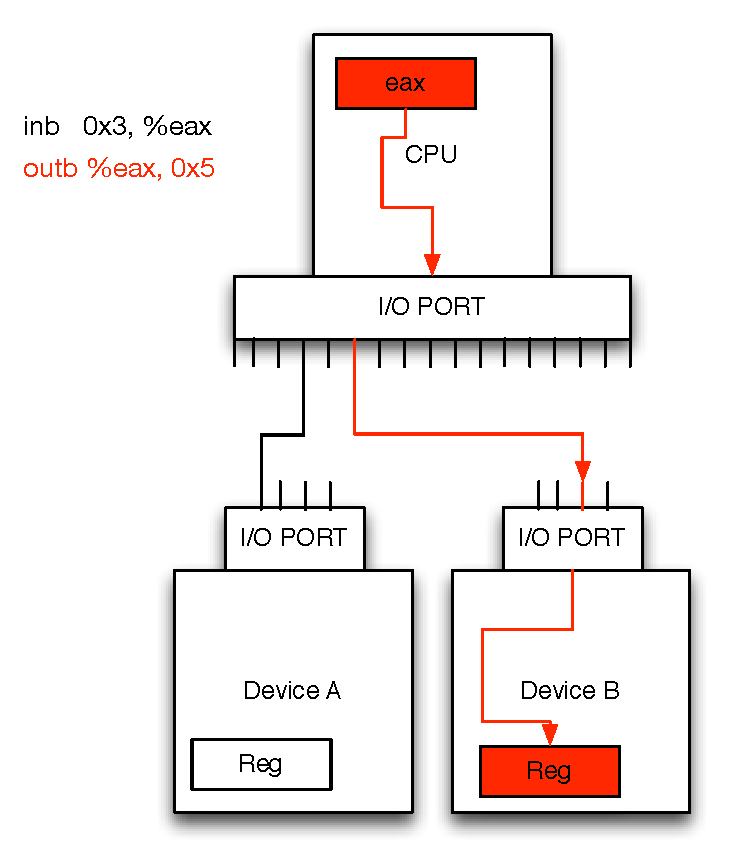
\includegraphics[height=225pt]{figures/ioport_3.pdf}}
\only<4>{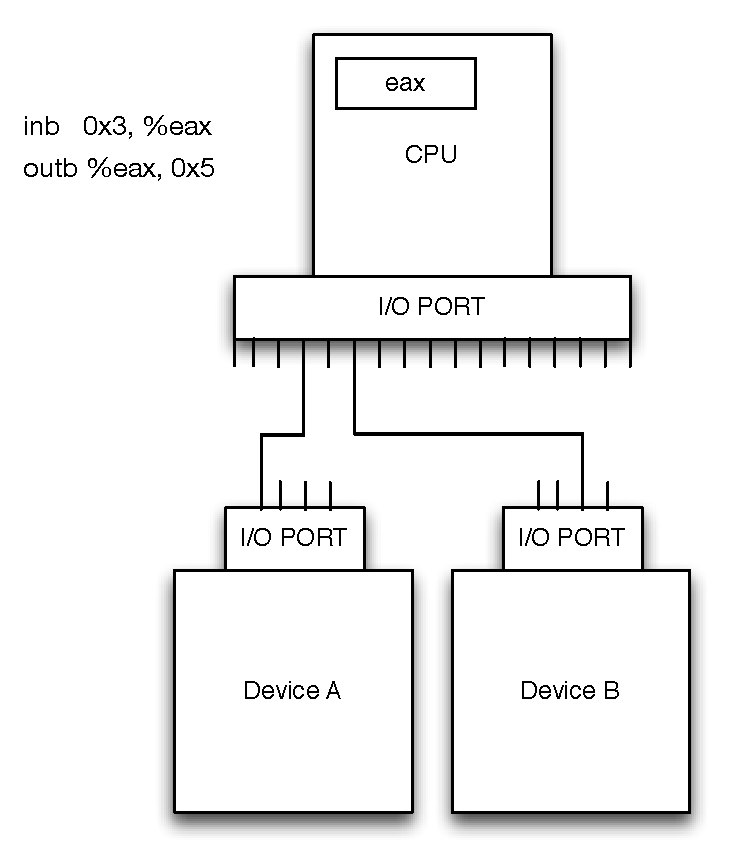
\includegraphics[height=225pt]{figures/ioport_4.pdf}}
\end{overlayarea}
\end{center}
\end{frame}

\subsection{MMIO}
\begin{frame}
        \frametitle{MMIO}
        \begin{itemize}
        \item Memory Mapped Input Output.
        \item It's a physicall address but it's not RAM.
        \item Can be mapped using pagination or segmentation.
        \item Can be cached, but be careful.
        \end{itemize}
\end{frame}

\begin{frame}
\begin{center}
\begin{overlayarea}{10cm}{10cm}
\only<1>{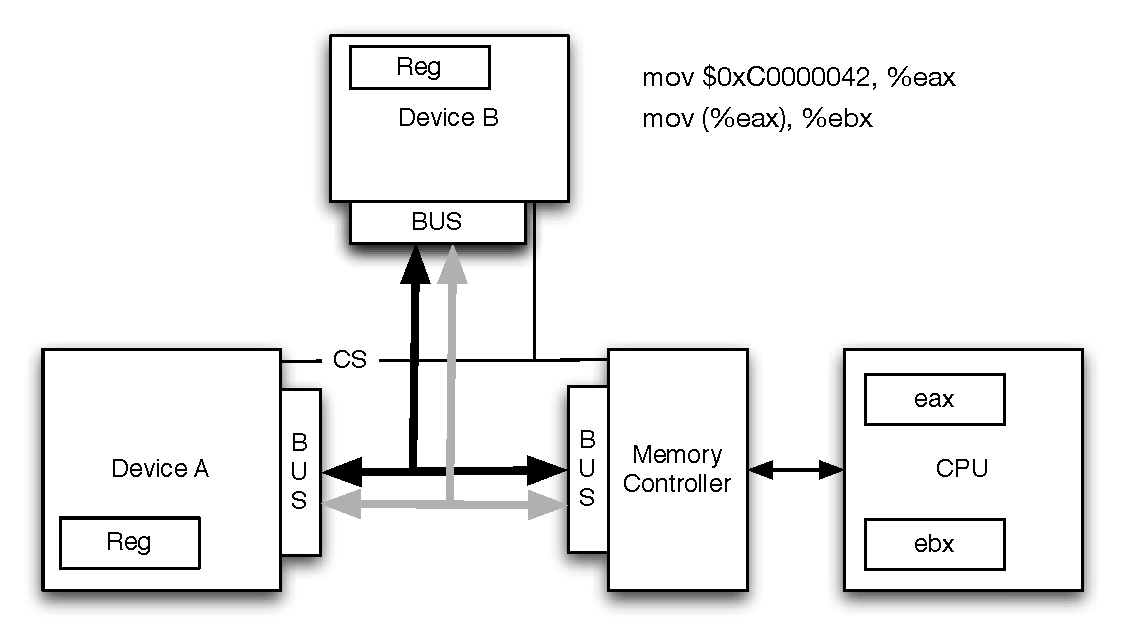
\includegraphics[height=150pt]{figures/mmio_1.pdf}}
\only<2>{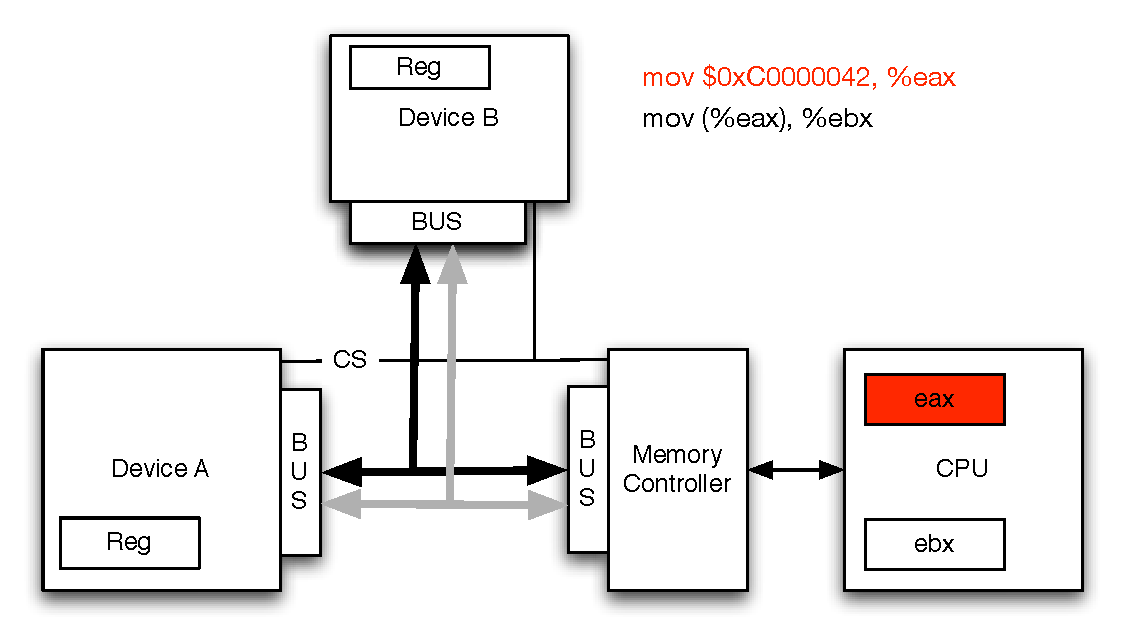
\includegraphics[height=150pt]{figures/mmio_2.pdf}}
\only<3>{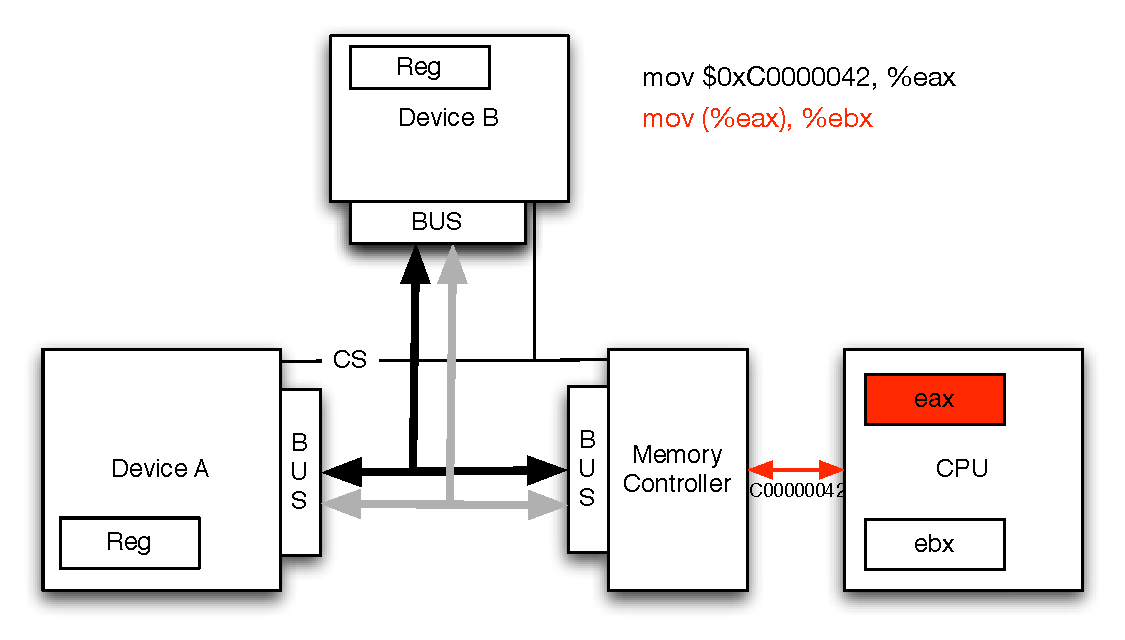
\includegraphics[height=150pt]{figures/mmio_3.pdf}}
\only<4>{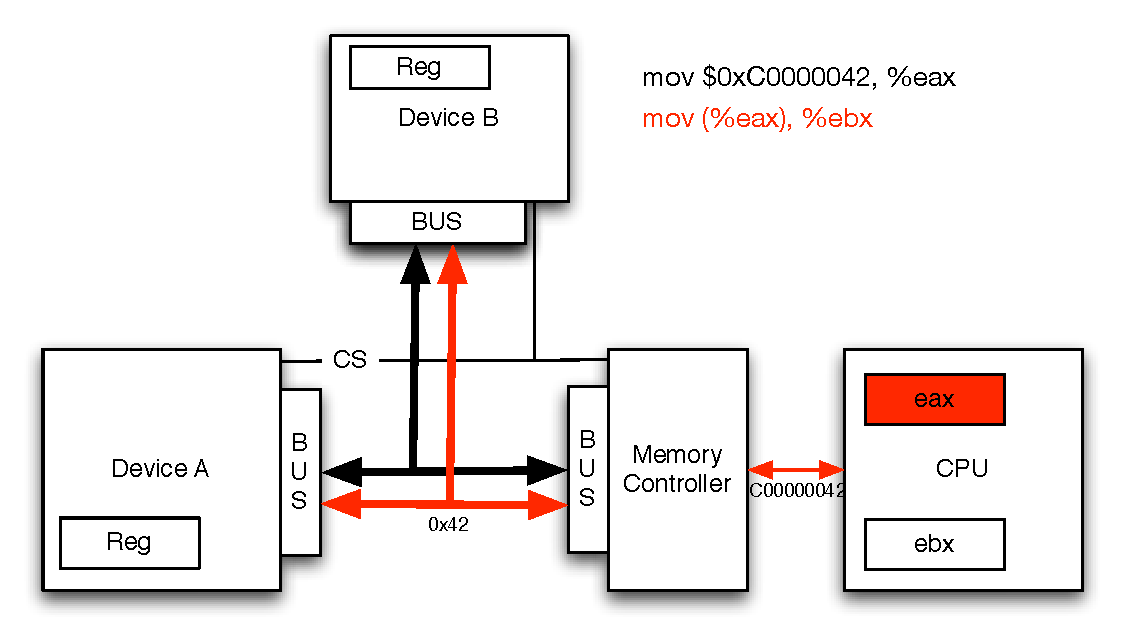
\includegraphics[height=150pt]{figures/mmio_4.pdf}}
\only<5>{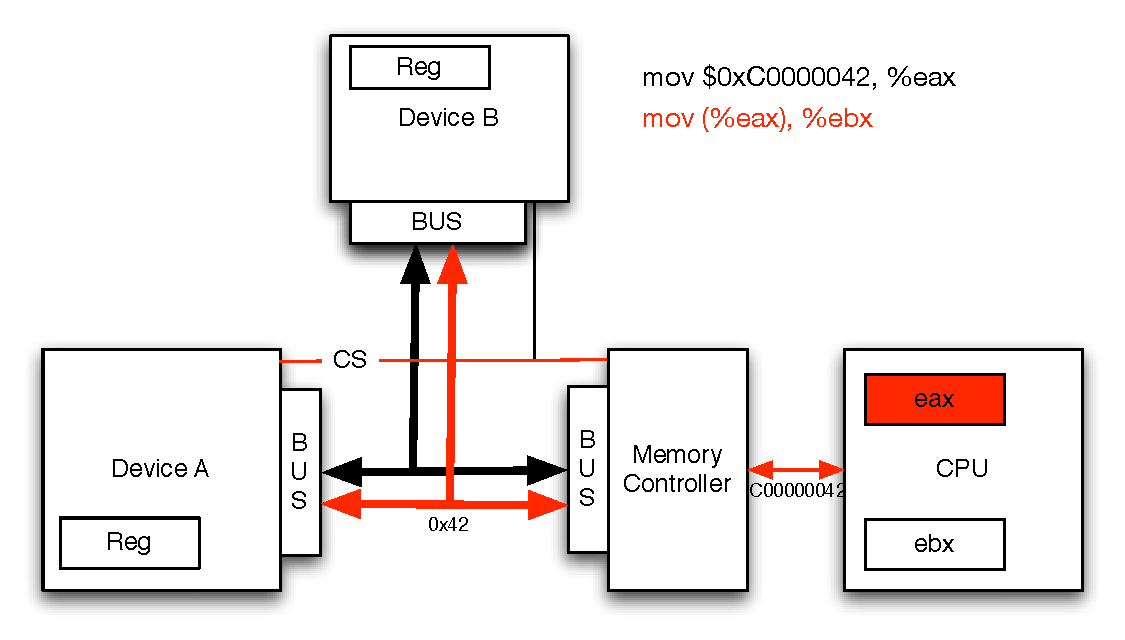
\includegraphics[height=150pt]{figures/mmio_5.pdf}}
\only<6>{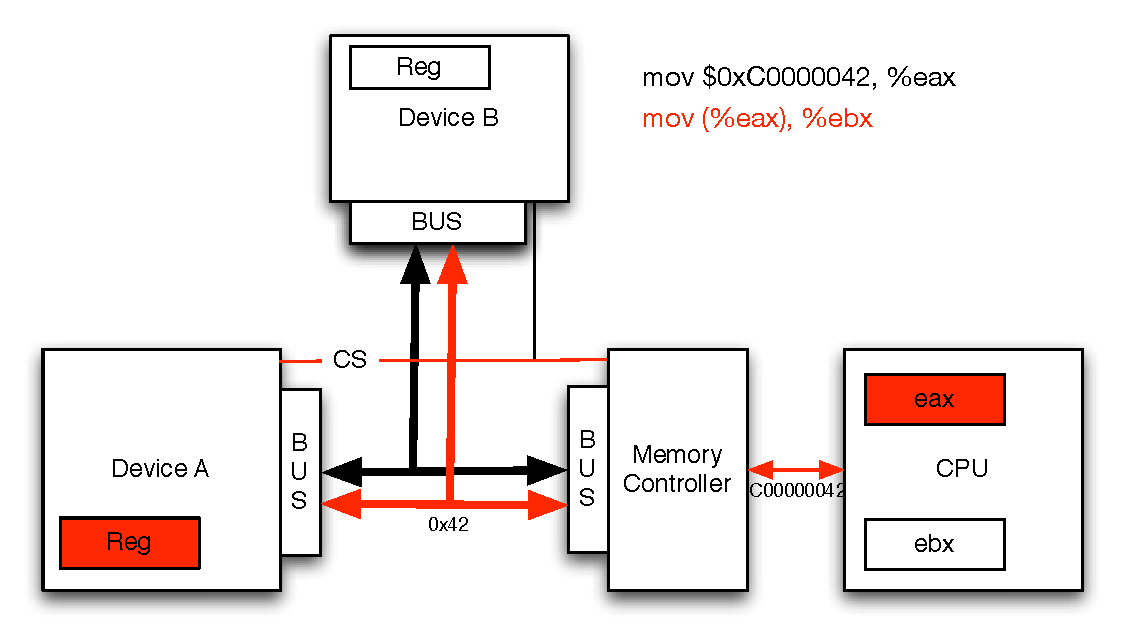
\includegraphics[height=150pt]{figures/mmio_6.pdf}}
\only<7>{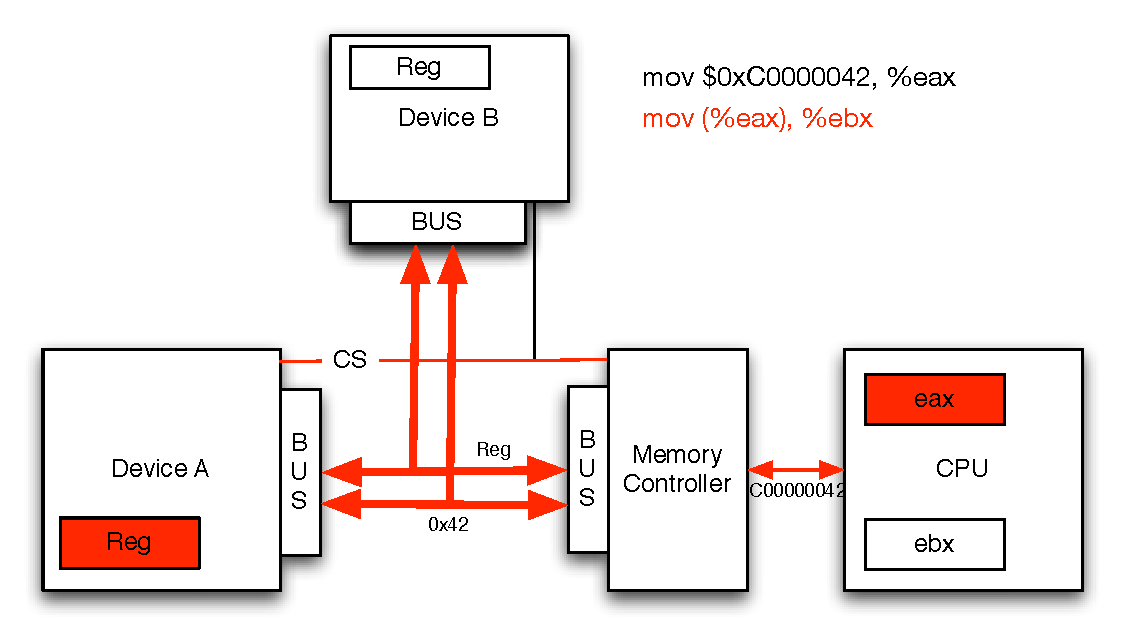
\includegraphics[height=150pt]{figures/mmio_7.pdf}}
\only<8>{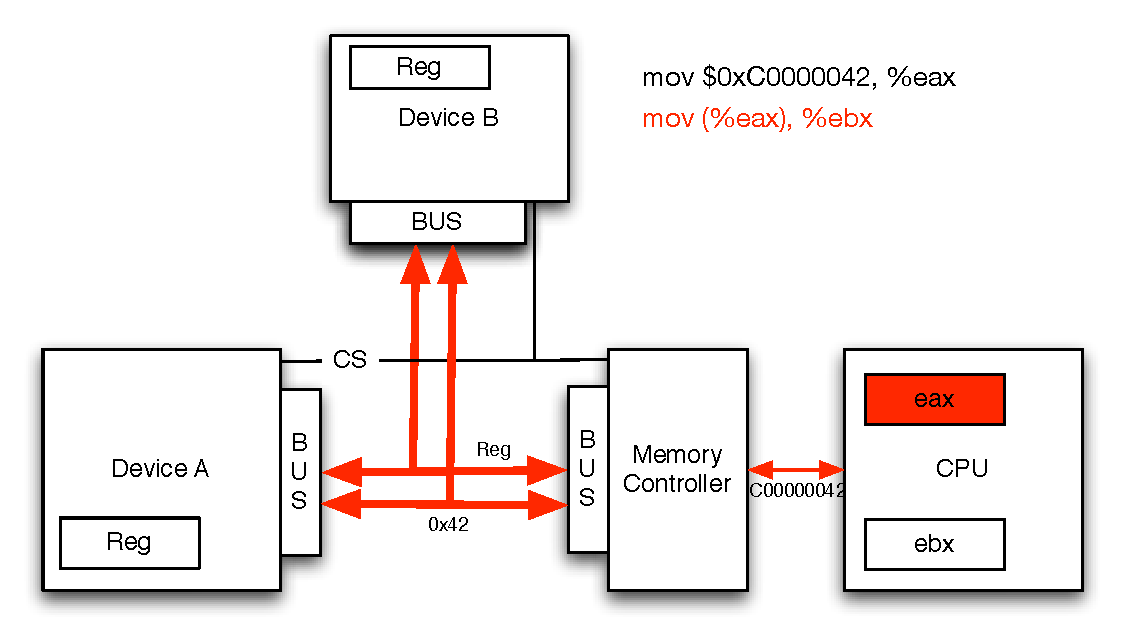
\includegraphics[height=150pt]{figures/mmio_8.pdf}}
\only<9>{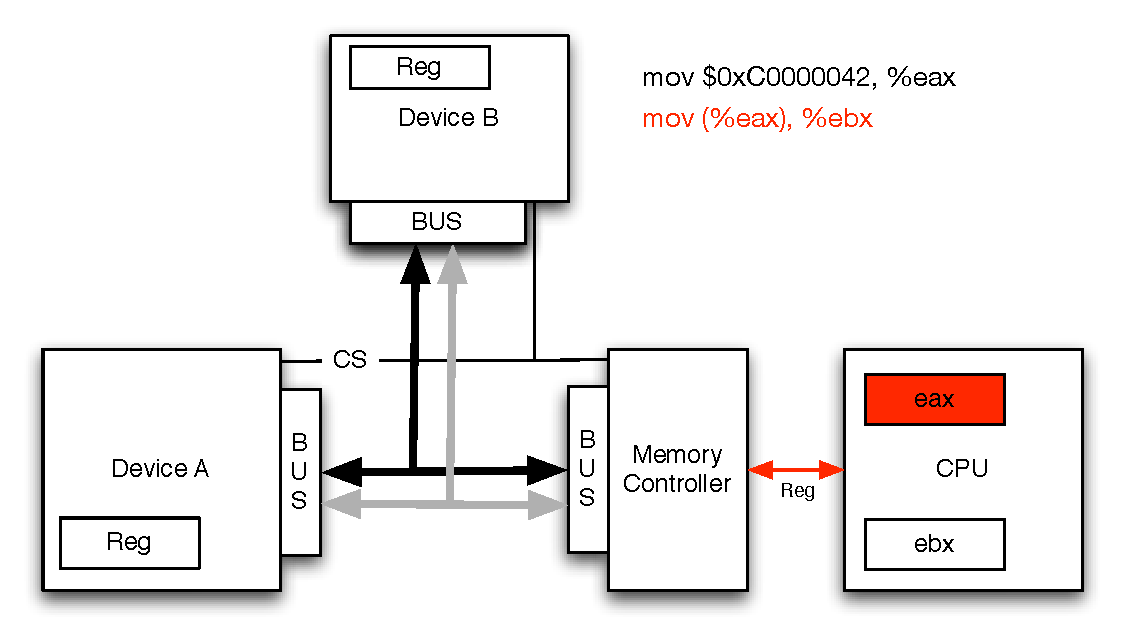
\includegraphics[height=150pt]{figures/mmio_9.pdf}}
\only<10>{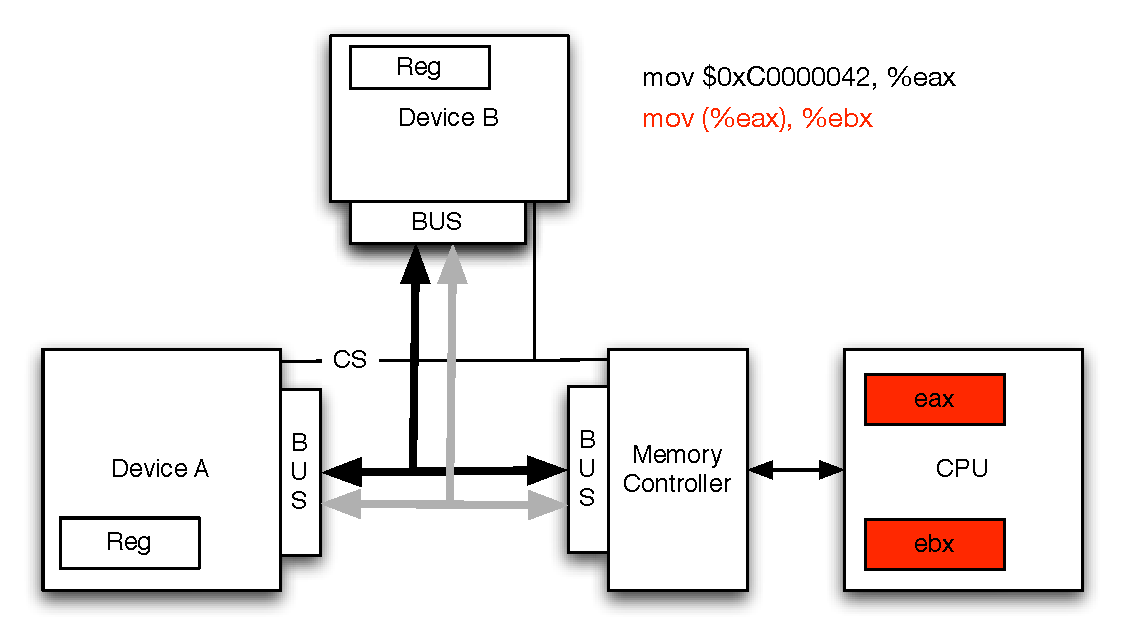
\includegraphics[height=150pt]{figures/mmio_10.pdf}}
\end{overlayarea}
\end{center}
\end{frame}

\subsection{DMA}
\begin{frame}
\frametitle{DMA}
        \begin{itemize}
        \item Direct Memory Access
        \item Background transfert from phys memory to phys memory.
        \item An interupt is raised when the transfert is done.
        \item Modern way to do big transfert.
        \end{itemize}
\end{frame}

\begin{frame}
\begin{center}
\begin{overlayarea}{10cm}{10cm}
\only<1>{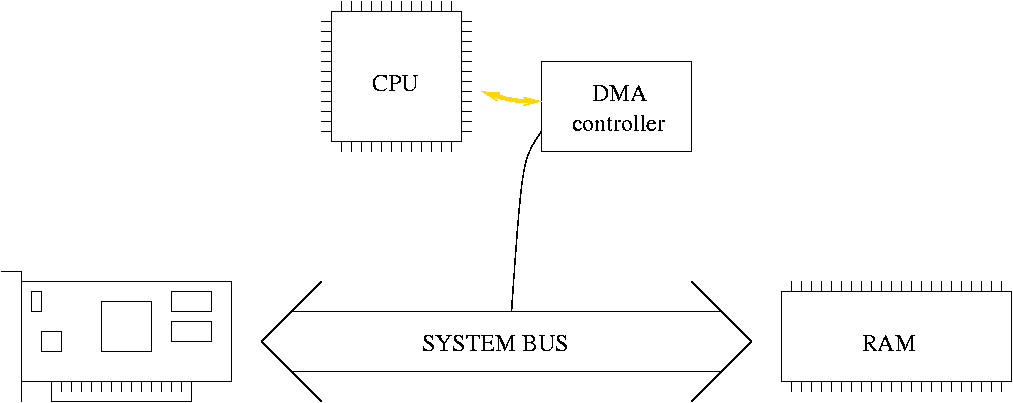
\includegraphics[height=150pt,width=302pt]{figures/dma-step1}}
\only<2>{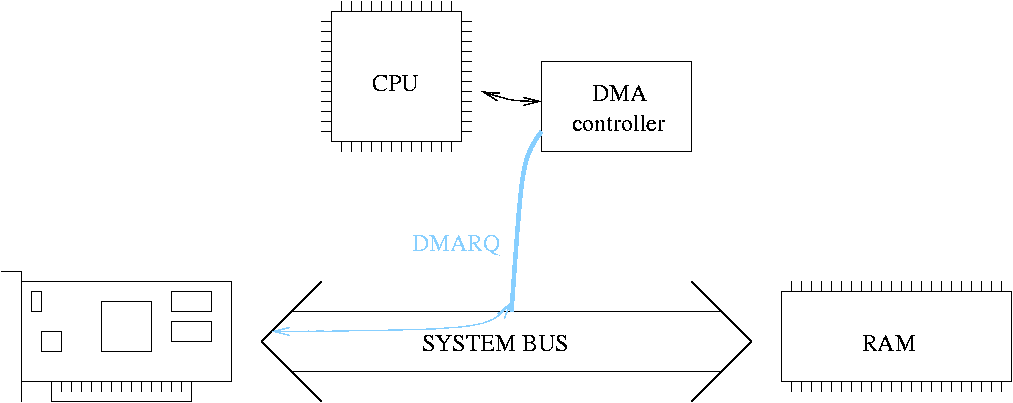
\includegraphics[height=150pt,width=302pt]{figures/dma-step2}}
\only<3>{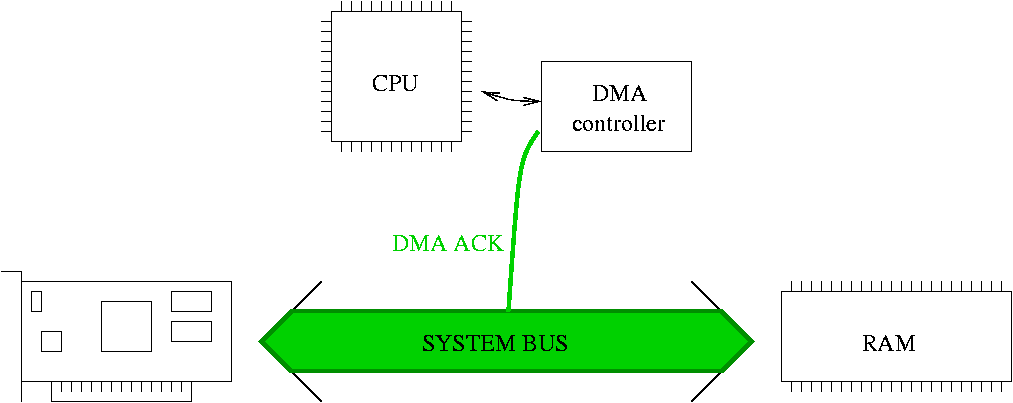
\includegraphics[height=150pt,width=302pt]{figures/dma-step3}}
\end{overlayarea}
\end{center}
\end{frame}

\section{Driver exemple, i8042}

\begin{frame}
\frametitle{Description}
\begin{itemize}
\item i8042 is the standar keyboard controller.
\item i8042 got 2 IO ports, 0x60 and 0x64.
\item 0x60 is the data port, 0x64 is the cmd port.
\item i8042 wired on the IRQ 1.
\end{itemize}
\end{frame}

\begin{frame}
\frametitle{Steps}
\begin{enumerate}
\item Received and interrupt.
\item Read status register (cmd).
\item Read data register.
\end{enumerate}
\end{frame}

\begin{frame}[fragile]
\frametitle{Exemple i8042}
\begin{verbatim}
void irq1_handler(void)
{
    uint8_t st;

    st = inb(0x64);
    if (st & 0x10 || st & 0x20)
       inb(0x60)
    else
      printf("Not a i8042 event\n");
}
\end{verbatim}
\end{frame}


\section{PCI Bus}
\subsection*{Background}
\begin{frame}
\frametitle{Background}
\begin{itemize}
\item PCI, Peripheral Component Interconnect
\item Different version exists:
\begin{itemize}
\item PCI 2.2 32 bits, 33MHz, 133 Mo/s.
\item PCI 2.2 64 bits, 64 MHz, 528 Mo/s.
\item PCI-X 64 bits, 133 MHz, 1066 Mo/s.
\end{itemize}
\item The bandwidth is shared between the devices on the same bus. That
why AGP has been created, to dedicate some bandwidth to the graphic
card.
\item In PCI express the bandwidth is not shared anymore. 
\item PCI is even used for internal device connexion in the southbridge
like (network card or sound card).
\end{itemize}
\end{frame}

\subsection{BDF, Bus Device Fonction}
\begin{frame}[fragile]
\frametitle{Bus Device Fonction}
This is the naming convention for pci device.

\-

00:12.4:
\begin{itemize}
\item Bus: 00
\item Device: 12
\item Function: 4
\end{itemize}

\-

A same device can expose mutiple functions, it's ofen the case for usb
controllers:

\begin{verbatim}
00:1d.0 USB Controller [0c03]:USB UHCI Controller #1 [8086:27c8]
00:1d.1 USB Controller [0c03]:USB UHCI Controller #2 [8086:27c9]
00:1d.2 USB Controller [0c03]:USB UHCI Controller #3 [8086:27ca]
00:1d.3 USB Controller [0c03]:USB UHCI Controller #4 [8086:27cb]
00:1d.7 USB Controller [0c03]:USB2 EHCI Controller [8086:27cc]
\end{verbatim}

\end{frame}

\subsection{Config Space and BAR}
\begin{frame}
\frametitle{Config space and BAR}
In order to configure, list, play with the pci devices. Each device got
there own configuration table, called Config space.

\-

The pci config space expose the different MMIO region and I/O port that
a specific device use. By default the pci space starts at 0x80000000,
but it can be remmaped.

\-

The pci BAR (Base address register), is an offset where to find the
memory region of the devices. This is where are the registers.

\end{frame}

\begin{frame}
\begin{center}
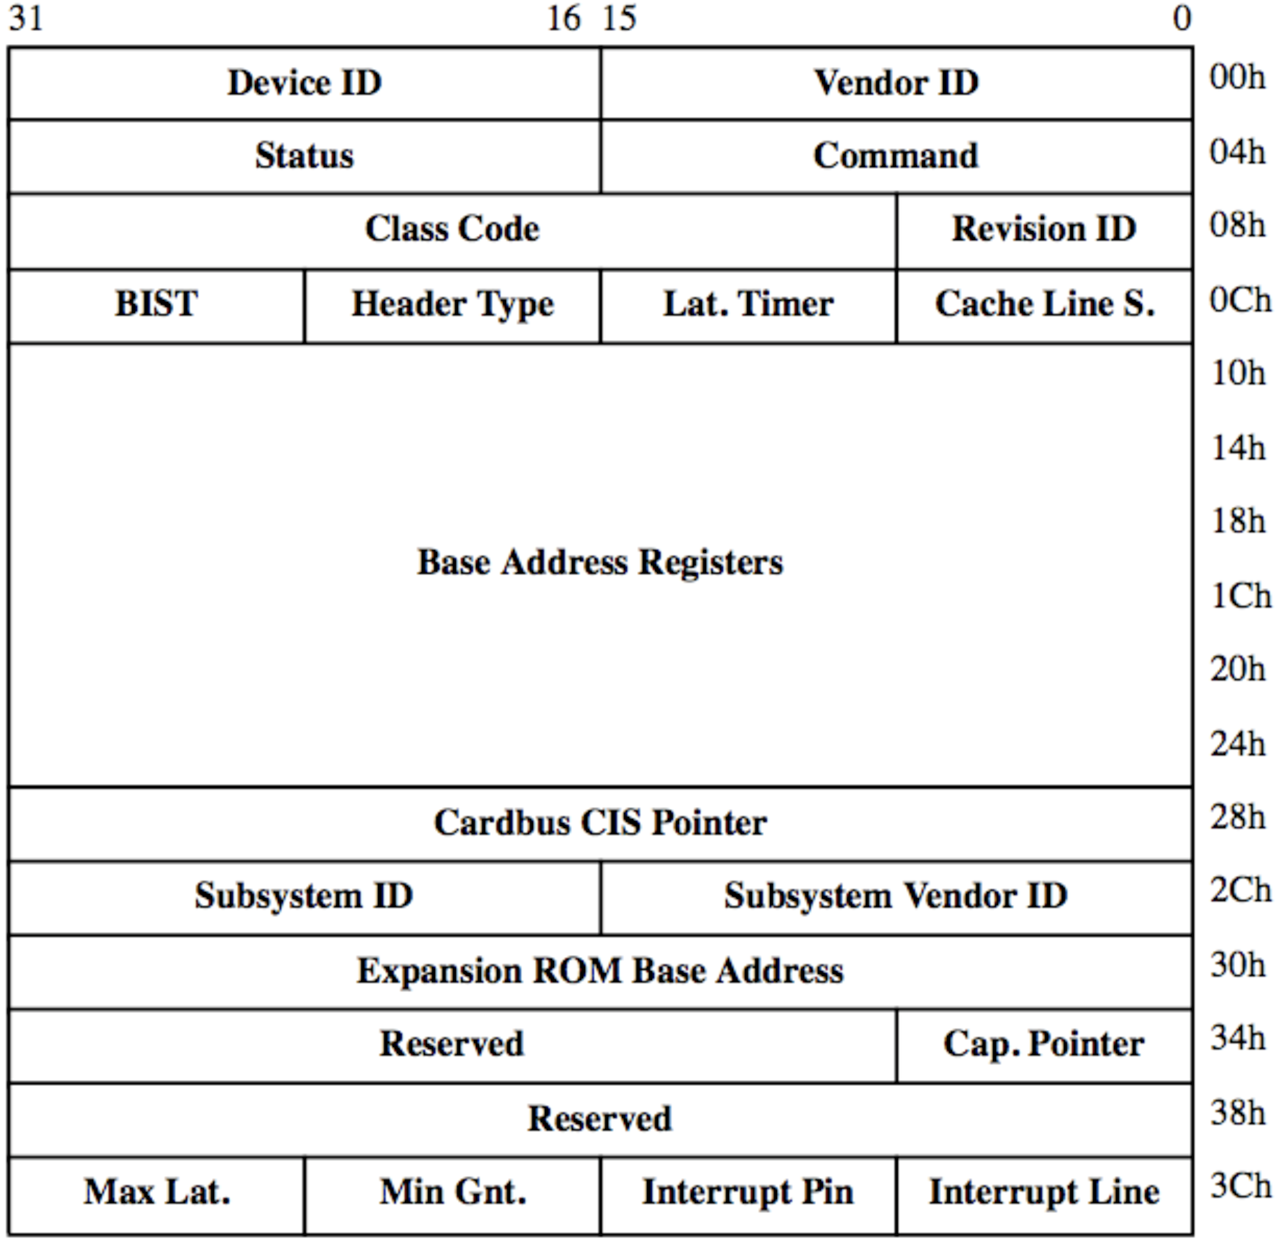
\includegraphics[height=150pt]{figures/config_space}
\end{center}
\end{frame}

\begin{frame}[fragile]
\frametitle{ATI graphic card exemple}
\begin{verbatim}
01:00.0 0300: 1002:7104 (prog-if 00 [VGA controller])
  Subsystem: 1002:0b32
  Control: I/O+ Mem+ BusMaster+ SpecCycle- MemWINV- VGASnoop- ParErr- Stepping- SERR- FastB2B- DisINTx-
  Status: Cap+ 66MHz- UDF- FastB2B- ParErr- DEVSEL=fast >TAbort- <TAbort- <MAbort- >SERR- <PERR- INTx-
  Latency: 0, Cache Line Size: 64 bytes
  Interrupt: pin A routed to IRQ 16
  Region 0: Memory at d0000000 (64-bit, prefetchable) [size=256M]
  Region 2: Memory at efde0000 (64-bit, non-prefetchable) [size=64K]
  Region 4: I/O ports at dc00 [size=256]
  Expansion ROM at efe00000 [disabled] [size=128K]
\end{verbatim}

\begin{verbatim}
00: 02 10 04 71 07 00 10 00 00 00 00 03 10 00 80 00
10: 0c 00 00 d0 00 00 00 00 04 00 de ef 00 00 00 00
20: 01 dc 00 00 00 00 00 00 00 00 00 00 02 10 32 0b
30: 00 00 e0 ef 50 00 00 00 00 00 00 00 0b 01 00 00
40: 00 00 00 00 00 00 00 00 00 00 00 00 02 10 32 0b
50: 01 58 02 06 00 00 00 00 10 80 01 00 a0 0f 64 08
60: 16 09 00 00 01 0d 00 00 40 00 01 11 00 00 00 00
70: 00 00 00 00 00 00 00 00 00 00 00 00 00 00 00 00
80: 05 00 80 00 00 00 00 00 00 00 00 00 00 00 00 00
90: 00 00 00 00 00 00 00 00 00 00 00 00 00 00 00 00
a0: 00 00 00 00 00 00 00 00 00 00 00 00 00 00 00 00
b0: 00 00 00 00 00 00 00 00 00 00 00 00 00 00 00 00
c0: 00 00 00 00 00 00 00 00 00 00 00 00 00 00 00 00
d0: 00 00 00 00 00 00 00 00 00 00 00 00 00 00 00 00
e0: 00 00 00 00 00 00 00 00 00 00 00 00 00 00 00 00
f0: 00 00 00 00 00 00 00 00 00 00 00 00 00 00 00 00
\end{verbatim}
\end{frame}

\section{USB}
\subsection*{Background}
\subsection{Protocoles}
\subsection{Transfert modes}
\subsection{UHCI}
\subsection{Futurs}

\end{document}
